% Fig 3 -- IRexp composition & technical validation (six-panel multiple).
% a Source  b Licence pool  c Modality linkage  d Band-count histogram
% e Elemental distribution (two-column hbars)  f Automated QC validation (2x2)
%
% Design notes (why the geometry looks the way it does):
%   pgfplots' `at`/`anchor` pair positions the PLOT BOX only; tick labels,
%   axis labels and titles are drawn OUTSIDE that box and are not counted
%   in `width`/`height`. In a dense small-multiples layout this means every
%   column needs an explicitly reserved margin for (i) its own outside
%   labels and (ii) any neighbour's value-label overflow, or panels bleed
%   into each other. Every column below therefore carries an explicit
%   "label zone" width and the xmax of every bar plot is pushed out ~20-30%
%   past the data max so in-panel value labels never need to leave the box.
\documentclass[border=0pt,tikz]{standalone}
% Nature Portfolio / Scientific Data shared TikZ style for IRexp figures.
% Width: 183 mm double-column. Typography: Helvetica-class (phv).
\RequirePackage{tikz}
\RequirePackage{pgfplots}
\RequirePackage{xcolor}
\RequirePackage{helvet}
\IfFileExists{sansmathfonts.sty}{\RequirePackage{sansmathfonts}}{}
\renewcommand{\familydefault}{\sfdefault}
\pgfplotsset{compat=1.18}
\usetikzlibrary{
  arrows.meta,calc,positioning,fit,shapes.geometric,shapes.misc,
  backgrounds,shadows.blur,patterns,decorations.pathreplacing
}

% ---- Paul Tol / NMRexp-matched palette ----
\definecolor{nmrBlue}{HTML}{4A7EBB}
\definecolor{nmrBlueDark}{HTML}{2E5F8F}
\definecolor{nmrBlueLight}{HTML}{A8C8E8}
\definecolor{nmrPeach}{HTML}{E8B48C}
\definecolor{nmrNavy}{HTML}{1B3D5C}
\definecolor{nmrRed}{HTML}{C44E52}
\definecolor{nmrGreen}{HTML}{3D8B5E}
\definecolor{nmrOrange}{HTML}{D97B32}
\definecolor{ink}{HTML}{1A1A1A}
\definecolor{muted}{HTML}{7A7F85}
\definecolor{note}{HTML}{5C636A}
\definecolor{faint}{HTML}{E8EAEC}
\definecolor{ghost}{HTML}{C5C9CD}
\definecolor{tintBlue}{HTML}{EEF3F8}
\definecolor{tintGreen}{HTML}{EAF4EE}

\newcommand{\NatureFont}{\fontfamily{phv}\selectfont}
\newcommand{\PanelLabel}[1]{%
  {\NatureFont\bfseries\fontsize{8}{9.6}\selectfont #1}%
}
\newcommand{\FigBody}{\NatureFont\fontsize{7}{8.4}\selectfont}
\newcommand{\FigSmall}{\NatureFont\fontsize{5.5}{6.6}\selectfont}
\newcommand{\FigAxis}{\NatureFont\fontsize{7}{8.4}\selectfont}

\tikzset{
  nature arrow/.style={
    -{Latex[length=1.6mm,width=1.3mm]},
    line width=0.55pt, ink
  },
  nature arrow grey/.style={
    -{Latex[length=1.6mm,width=1.3mm]},
    line width=0.5pt, note
  },
  stage card/.style={
    draw=nmrBlueDark, line width=0.7pt, rounded corners=2.2pt,
    fill=white, inner sep=3pt, align=center, font=\FigBody
  },
  stage header/.style={
    fill=nmrBlueDark, text=white, font=\FigBody\bfseries,
    rounded corners=2.2pt, inner sep=2.5pt, align=center
  },
  soft card/.style={
    draw=ghost, line width=0.55pt, rounded corners=2.2pt,
    fill=white, inner sep=3.5pt, align=left, font=\FigBody
  },
}

\pgfplotsset{
  nature axis/.style={
    tick label style={font=\FigSmall, /pgf/number format/assume math mode},
    label style={font=\FigAxis\bfseries},
    title style={font=\FigBody\bfseries, color=ink},
    axis line style={ink, line width=0.5pt},
    tick style={ink, line width=0.45pt},
    major grid style={faint, line width=0.35pt},
    axis x line=bottom,
    axis y line=left,
    enlarge x limits=false,
    clip=false,
  },
  nature hbar/.style={
    nature axis,
    xbar,
    bar width=7pt,
    y=data,
    nodes near coords,
    every node near coord/.append style={
      font=\FigSmall, ink, anchor=west, /pgf/number format/fixed,
      /pgf/number format/1000 sep={,}
    },
    xtick=\empty,
    axis x line=none,
    y axis line style={ink, line width=0.55pt},
    ytick style={draw=none},
    y tick label style={font=\FigBody, ink, anchor=east},
    grid=major x,
    xmin=0,
  },
}


\pgfplotsset{
  irx hbar/.style={
    nature axis,
    xbar, bar width=6.2pt,
    axis x line=none, axis y line=left,
    y axis line style={ink, line width=0.55pt, -},
    tick style={draw=none},
    y tick label style={font=\FigBody, ink, anchor=east, align=right, text width=18mm},
    nodes near coords,
    every node near coord/.append style={
      font=\FigSmall, ink, anchor=west,
      /pgf/number format/fixed, /pgf/number format/1000 sep={,}
    },
    xmin=0, clip=false,
  },
  irx hbar narrow/.style={
    nature axis,
    xbar, bar width=3.4pt,
    axis x line=none, axis y line=left,
    y axis line style={ink, line width=0.5pt, -},
    tick style={draw=none},
    y tick label style={font=\FigSmall, ink, anchor=east},
    nodes near coords,
    every node near coord/.append style={
      font=\FigSmall, ink, anchor=west,
      /pgf/number format/fixed, /pgf/number format/1000 sep={,}
    },
    xmin=0, clip=false,
  },
  irx vbar/.style={
    nature axis,
    ybar, bar width=2.6pt,
    axis y line=left, axis x line=bottom,
    x axis line style={ink, line width=0.5pt, -},
    y axis line style={ink, line width=0.5pt, -},
    tick style={ink, line width=0.4pt},
    xlabel style={font=\FigSmall, ink},
    ylabel style={font=\FigSmall, ink},
    tick label style={font=\FigSmall, /pgf/number format/fixed, /pgf/number format/1000 sep={,}},
    scaled y ticks=false, scaled x ticks=false,
    xmin=2, ymin=0, enlarge x limits=0.03, clip=false,
  },
  irx qc/.style={
    nature axis,
    ybar interval, bar width=0pt,
    axis y line=left, axis x line=bottom,
    x axis line style={ink, line width=0.45pt, -},
    y axis line style={ink, line width=0.45pt, -},
    tick style={ink, line width=0.35pt},
    tick label style={font=\FigSmall},
    xlabel style={font=\FigSmall, ink, yshift=1pt},
    ylabel style={font=\FigSmall, ink},
    ymin=0, enlarge x limits=0, clip=false,
    title style={font=\FigBody\bfseries, ink, yshift=-1pt},
  },
}

% L-shaped leader line: bar top (#1,#2) up/down to shelf, then across to (#3,#4)
\newcommand{\Elbow}[4]{\draw[muted, line width=0.35pt] (axis cs:#1,#2) -- (axis cs:#1,#4) -- (axis cs:#3,#4);}

\begin{document}
\NatureFont
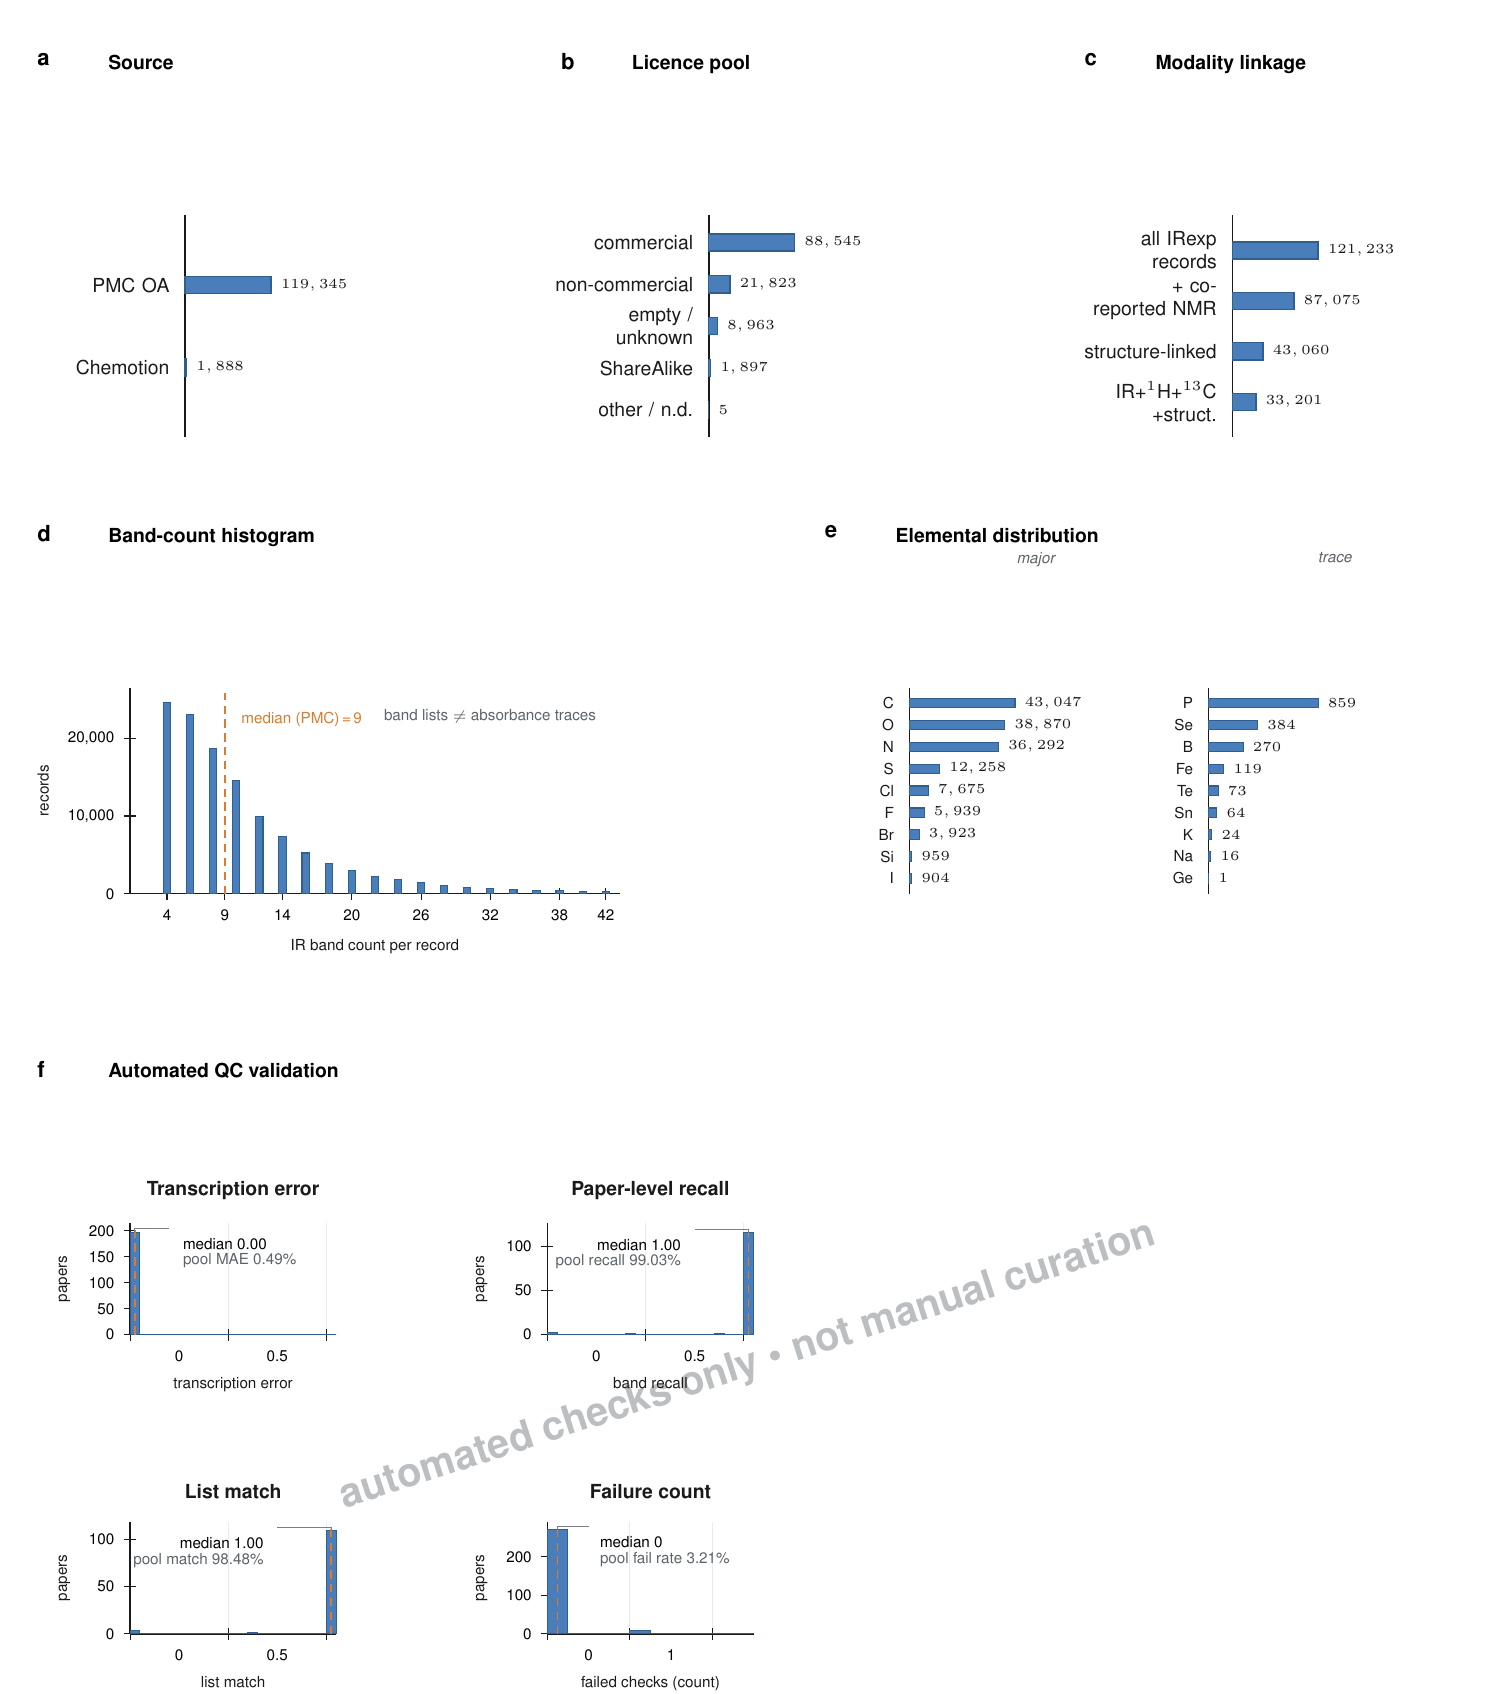
\begin{tikzpicture}[x=1mm,y=1mm]
\useasboundingbox (0,0) rectangle (183,208);

% ===========================================================================
% Row 1 -- a Source | b Licence pool | c Modality linkage  (hbar triptych)
% ===========================================================================
\def\RowOneAxisY{156}
\def\RowOneLabelY{206}
\def\RowOneH{44mm}
\def\RowOnePlotW{30mm}
\def\PaX{0}
\def\PbX{66.5}
\def\PcX{133}
\pgfmathsetmacro{\PaBoxX}{\PaX+20}
\pgfmathsetmacro{\PbBoxX}{\PbX+20}
\pgfmathsetmacro{\PcBoxX}{\PcX+20}

\node[anchor=north west] at (\PaX,\RowOneLabelY) {\PanelLabel{a}};
\node[font=\FigAxis,anchor=north west,align=left] at (\PaX+9,\RowOneLabelY-0.3) {\bfseries Source};
\node[anchor=north west] at (\PbX,\RowOneLabelY) {\PanelLabel{b}};
\node[font=\FigAxis,anchor=north west,align=left] at (\PbX+9,\RowOneLabelY-0.3) {\bfseries Licence pool};
\node[anchor=north west] at (\PcX,\RowOneLabelY) {\PanelLabel{c}};
\node[font=\FigAxis,anchor=north west,align=left] at (\PcX+9,\RowOneLabelY-0.3) {\bfseries Modality linkage};

% --- a: Source (PMC OA vs Chemotion) ---
\begin{axis}[irx hbar, width=\RowOnePlotW, height=\RowOneH, at={(\PaBoxX mm,\RowOneAxisY mm)}, anchor=south west,
  ymin=-0.85,ymax=1.85, ytick={0,1}, yticklabels={Chemotion,{PMC OA}}, xmax=155000]
\addplot[fill=nmrBlue,draw=nmrBlueDark,line width=0.5pt]
  coordinates {(119345,1) (1888,0)};
\end{axis}

% --- b: Licence pool ---
\begin{axis}[irx hbar, width=\RowOnePlotW, height=\RowOneH, at={(\PbBoxX mm,\RowOneAxisY mm)}, anchor=south west,
  ymin=-0.65,ymax=4.65, ytick={0,1,2,3,4},
  yticklabels={{other / n.d.},ShareAlike,{empty / unknown},non-commercial,commercial},
  xmax=115000]
\addplot[fill=nmrBlue,draw=nmrBlueDark,line width=0.5pt]
  coordinates {(88545,4) (21823,3) (8963,2) (1897,1) (5,0)};
\end{axis}

% --- c: Modality linkage ---
\begin{axis}[irx hbar, width=\RowOnePlotW, height=\RowOneH, at={(\PcBoxX mm,\RowOneAxisY mm)}, anchor=south west,
  ymin=-0.7,ymax=3.7, ytick={0,1,2,3},
  yticklabels={{IR+$^1$H+$^{13}$C\\+struct.},{structure-linked},
               {+ co-reported NMR},{all IRexp records}},
  xmax=158000]
\addplot[fill=nmrBlue,draw=nmrBlueDark,line width=0.5pt]
  coordinates {(121233,3) (87075,2) (43060,1) (33201,0)};
\end{axis}

% ===========================================================================
% Row 2 -- d Band-count histogram | e Elemental distribution (two columns)
% ===========================================================================
\def\RowTwoLabelY{146}
\def\RowTwoAxisY{98}
\def\RowTwoH{42mm}

\node[anchor=north west] at (0,\RowTwoLabelY) {\PanelLabel{d}};
\node[font=\FigAxis,anchor=north west,align=left] at (9,\RowTwoLabelY-0.3) {\bfseries Band-count histogram};
\node[anchor=north west] at (100,\RowTwoLabelY) {\PanelLabel{e}};
\node[font=\FigAxis,anchor=north west,align=left] at (109,\RowTwoLabelY-0.3) {\bfseries Elemental distribution};

% --- d: band-count histogram, honest linear y, PMC median annotated ---
\begin{axis}[irx vbar, width=78mm, height=\RowTwoH, at={(13mm,\RowTwoAxisY mm)}, anchor=south west,
  xlabel={IR band count per record}, ylabel={records},
  xtick={4,9,14,20,26,32,38,42}, ymax=26500]
\addplot[fill=nmrBlue,draw=nmrBlueDark,line width=0.4pt]
 coordinates {(4,24556)(6,22989)(8,18726)(10,14534)(12,9959)(14,7368)(16,5241)
 (18,3899)(20,3017)(22,2202)(24,1822)(26,1426)(28,1069)(30,826)(32,698)(34,534)
 (36,386)(38,408)(40,298)(42,250)};
\draw[nmrOrange,densely dashed,line width=0.7pt] (axis cs:9,0) -- (axis cs:9,25800);
\node[font=\FigSmall,text=nmrOrange,anchor=south west] at (axis cs:9.6,20200) {median (PMC)\,=\,9};
\node[font=\FigSmall,text=note,anchor=north east,align=right] at (axis cs:42,25000)
  {band lists $\neq$ absorbance traces};
\end{axis}

% --- e: elemental distribution, split into major / trace columns (both linear) ---
\begin{axis}[irx hbar narrow, width=32mm, height=\RowTwoH, at={(112mm,\RowTwoAxisY mm)}, anchor=south west,
  ymin=-0.7,ymax=8.7, ytick={0,...,8}, xmax=52000,
  yticklabels={I,Si,Br,F,Cl,S,N,O,C}]
\addplot[fill=nmrBlue,draw=nmrBlueDark,line width=0.4pt]
 coordinates {(43047,8)(38870,7)(36292,6)(12258,5)(7675,4)(5939,3)(3923,2)(959,1)(904,0)};
\end{axis}
\begin{axis}[irx hbar narrow, width=32mm, height=\RowTwoH, at={(150mm,\RowTwoAxisY mm)}, anchor=south west,
  ymin=-0.7,ymax=8.7, ytick={0,...,8}, xmax=1000,
  yticklabels={Ge,Na,K,Sn,Te,Fe,B,Se,P}]
\addplot[fill=nmrBlue,draw=nmrBlueDark,line width=0.4pt]
 coordinates {(1,0)(16,1)(24,2)(64,3)(73,4)(119,5)(270,6)(384,7)(859,8)};
\end{axis}
\node[font=\FigSmall,text=note,anchor=north,align=center] at (128,142.6)
  {\itshape major}; % subtle column caption above the split
\node[font=\FigSmall,text=note,anchor=north,align=center] at (166,142.6)
  {\itshape trace};

% ===========================================================================
% Row 3 -- f Automated QC validation (2x2 histogram grid)
% ===========================================================================
\def\RowThreeLabelY{78}
\def\SubRowOneY{42}
\def\SubRowTwoY{4}
\def\SubH{30mm}
\def\SubW{42mm}

\node[anchor=north west] at (0,\RowThreeLabelY) {\PanelLabel{f}};
\node[font=\FigAxis,anchor=north west,align=left] at (9,\RowThreeLabelY-0.3) {\bfseries Automated QC validation};
\node[muted,font=\FigSmall,rotate=18,opacity=0.5] at (91.5,\SubRowOneY-4)
  {\Large\bfseries automated checks only \textbullet\ not manual curation};

% --- f1: transcription error ---
\begin{axis}[irx qc, width=\SubW, height=\SubH, at={(13mm,\SubRowOneY mm)}, anchor=south west,
  xlabel={transcription error}, ylabel={papers}, title={Transcription error},
  xtick={0,0.5,1.0}, ymax=215]
\addplot[fill=nmrBlue,draw=nmrBlueDark,line width=0.35pt]
 coordinates {(0,196)(0.05,0)(0.1,0)(0.15,0)(0.2,0)(0.25,0)(0.3,0)(0.35,0)(0.4,1)(0.45,0)
 (0.5,1)(0.55,1)(0.6,0)(0.65,0)(0.7,0)(0.75,1)(0.8,0)(0.85,0)(0.9,0)(0.95,0)(1.0,0)(1.05,0)};
\draw[nmrOrange,densely dashed,line width=0.6pt] (axis cs:0.025,0) -- (axis cs:0.025,205);
\Elbow{0.025}{196}{0.20}{205}
\node[font=\FigSmall,anchor=north west,align=left] at (axis cs:0.22,205)
  {median 0.00\\[-1pt]\textcolor{note}{pool MAE 0.49\%}};
\end{axis}

% --- f2: paper-level band recall ---
\begin{axis}[irx qc, width=\SubW, height=\SubH, at={(66mm,\SubRowOneY mm)}, anchor=south west,
  xlabel={band recall}, ylabel={papers}, title={Paper-level recall},
  xtick={0,0.5,1.0}, ymax=126]
\addplot[fill=nmrBlue,draw=nmrBlueDark,line width=0.35pt]
 coordinates {(0,3)(0.05,0)(0.1,0)(0.15,0)(0.2,0)(0.25,0)(0.3,0)(0.35,0)(0.4,1)(0.45,0)
 (0.5,0)(0.55,0)(0.6,0)(0.65,0)(0.7,0)(0.75,0)(0.8,0)(0.85,1)(0.9,0)(0.95,0)(1.0,115)(1.05,0)};
\draw[nmrOrange,densely dashed,line width=0.6pt] (axis cs:1.025,0) -- (axis cs:1.025,119);
\Elbow{1.025}{115}{0.75}{119}
\node[font=\FigSmall,anchor=north east,align=right] at (axis cs:0.73,119)
  {median 1.00\\[-1pt]\textcolor{note}{pool recall 99.03\%}};
\end{axis}

% --- f3: list match ---
\begin{axis}[irx qc, width=\SubW, height=\SubH, at={(13mm,\SubRowTwoY mm)}, anchor=south west,
  xlabel={list match}, ylabel={papers}, title={List match}, xtick={0,0.5,1.0}, ymax=118]
\addplot[fill=nmrBlue,draw=nmrBlueDark,line width=0.35pt]
 coordinates {(0,4)(0.05,0)(0.1,0)(0.15,0)(0.2,0)(0.25,0)(0.3,0)(0.35,0)(0.4,0)(0.45,0)
 (0.5,1)(0.55,0)(0.6,2)(0.65,1)(0.7,1)(0.75,0)(0.8,1)(0.85,0)(0.9,0)(0.95,0)(1.0,109)(1.05,0)};
\draw[nmrOrange,densely dashed,line width=0.6pt] (axis cs:1.025,0) -- (axis cs:1.025,112);
\Elbow{1.025}{109}{0.75}{112}
\node[font=\FigSmall,anchor=north east,align=right] at (axis cs:0.73,112)
  {median 1.00\\[-1pt]\textcolor{note}{pool match 98.48\%}};
\end{axis}

% --- f4: failure count per check-run ---
\begin{axis}[irx qc, width=\SubW, height=\SubH, at={(66mm,\SubRowTwoY mm)}, anchor=south west,
  xlabel={failed checks (count)}, ylabel={papers}, title={Failure count}, xtick={0,1,2}, ymax=290]
\addplot[fill=nmrBlue,draw=nmrBlueDark,line width=0.35pt]
 coordinates {(0,271)(0.25,0)(0.5,0)(0.75,0)(1.0,9)(1.25,0)(1.5,0)(1.75,0)(2.0,0)(2.25,0)(2.5,0)};
\draw[nmrOrange,densely dashed,line width=0.6pt] (axis cs:0.125,0) -- (axis cs:0.125,278);
\Elbow{0.125}{271}{0.5}{278}
\node[font=\FigSmall,anchor=north west,align=left] at (axis cs:0.52,278)
  {median 0\\[-1pt]\textcolor{note}{pool fail rate 3.21\%}};
\end{axis}

\end{tikzpicture}
\end{document}
